% a-project.tex, v-1.0.3 marcoreis baseado no
% abntex2-modelo-trabalho-academico.tex, v-1.9.7 laurocesar
% Copyright 2012-2018 by abnTeX2 group at http://www.abntex.net.br/ 
% 
% This work consists of the files ........
% 
% -----------------------------------------------------------------------------
% Modelo para desenvolvimento de documentação de projetos acadêmicos
% (tese de doutorado, dissertação de mestrado e trabalhos de monografias em geral) 
% em conformidade com ABNT NBR 14724:2011: Informação e documentação. 
% -----------------------------------------------------------------------------
% Opções para a documentação
%
% Fancy page headings 
%\documentclass[fancyheadings, subook]{Classes/a-prj}
%\documentclass[fancyheadings, sureport]{Classes/a-prj}
%
% Fancy chapters and sections headings 
%\documentclass[fancychapter, subook]{Classes/a-prj}
%\documentclass[fancychapter, sureport]{Classes/a-prj}
%
% Fancy page , chapters and sections headings
%\documentclass[fancyheadings, fancychapter, subook]{Classes/a-prj}
\documentclass[fancyheadings, fancychapter, sureport]{Classes/a-prj}
%
% -----------------------------------------------------------------------------
% Alguns comandos para a fancy page headings)
%
% Page header line width
%\footlinewidth{value}
%
% Page footer line width
%\headlinewidth{value}
%
% Page header and footer line width
%\headingslinewidth{value}
%
% Page header and footer lines without text
%\headingslinesonly
%
% The default line width is 0.3pt.
% Set the value to 0pt to remove the page header and/or footer line
%
% -------------------------------------------------------------------------------
% Formato de figuras suportado
% -------------------------------------------------------------------------------
% O formato das figuras depende da forma como o arquivo de saída é gerado.
% As figuras inseridas na pasta Figures serão automaticamente reconhecidas sem
% a necessidade de inserir a extensão do arquivo.
%
% O pdfLaTEX (PDF) suporta figuras com as extensões: pdf, jpg, png e mps.
%
% -------------------------------------------------------------------------------
% Árvore do diretório a-project.tex
%  Diretório
%       \Classes        (requerido)
%       \Figures        (requerido) --------------------------------->
%       \Figures\PDF    (optional)
%       \Figures\JPG    (optional) Figures located within these
%       \Figures\PNG    (optional) folders are searched automatically
%       \Figures\MPS    (optional)  by the a-prj class.
%       \Figures\EPS    (optional)
%       \Figures\PS     (optional) <--------------------------------
%       \Tables         (requerido)
%       \Others         (requerido)
%       \Chapters       (requerido)
%       \Appendices     (optional)
%       \References     (requerido)
%
% -------------------------------------------------------------------------------
% PDF File resumo
\ifpdf
    \hypersetup{
    	backref,
        colorlinks  = true,
        pdftitle    = Modelo de documentação,
        pdfauthor   = {Marco Reis, marco.a.reis@gmail.com},
        pdfsubject  = Mestre em Engenharia,
        pdfcreator  = Subtitulo,
        pdfproducer = PDFLatex,
        pdfkeywords = {documentação, latex, dissertação, tese}}
 \fi
%
% -------------------------------------------------------------------------------
% Relação de pacotes opcionais utilizados
\usepackage[utf8]{inputenc}
\usepackage[brazil]{babel}
\usepackage{longtable}
\usepackage{dcolumn}
\usepackage{multirow}
\usepackage{lscape}
%\usepackage{graphicx}
\usepackage{rotating}
%\usepackage{float,subfigure}
%\usepackage{graphicx, subfigure}
\usepackage{cite}
\usepackage[left=3cm,top=3cm,right=2cm,bottom=2cm]{geometry}
\usepackage[alf]{abntex2cite}
\usepackage{ifpdf}
\usepackage{shadow}
\usepackage{wrapfig}
\usepackage[normalem]{ulem}
\usepackage{makeidx}
\usepackage{yfonts}
\usepackage{algorithm}
\usepackage{algorithmic}
\usepackage{lmodern}
\usepackage[T1]{fontenc}
\usepackage{indentfirst}
\usepackage{color}
\usepackage{microtype}
\usepackage{lipsum}
\usepackage{caption}
\usepackage{subcaption}
\usepackage{pdfpages}
%
\makeindex 
\setlength{\LTcapwidth}{\textwidth}
%
\newtheorem{theorem}{Teorema}
\newtheorem{definition}[theorem]{Definição}
%
% -------------------------------------------------------------------------------
% Configurações do pacote backref
\renewcommand{\backrefpagesname}{Citado na(s) página(s):~}
% Texto padrão antes do número das páginas
\renewcommand{\backref}{}
% Define os textos da citação
\renewcommand*{\backrefalt}[4]{
	\ifcase #1 %
		Nenhuma citação no texto.%
	\or
		Citado na página #2.%
	\else
		Citado #1 vezes nas páginas #2.%
	\fi
}
% 
% -------------------------------------------------------------------------------
% Início do documento raiz
\begin{document}
% Definição do título da página
    \university{Centro Universitário SENAI CIMATEC}
	%\faculty{Programa de...}
	%\school{Escola de...}
% 
    %\course{Engenharia Elétrica}
    \typework{Pós-Graduação em Robótica e Sistemas Autônomos}
% 
	%\course{Mestrado em Modelagem Computacional e Tecnologia Industrial}
	%\typework{Disserta\c{c}\~ao de mestrado}
	%\typework{Exame de Qualificação de Mestrado}
% 
	%\course{Engenharia Elétrica}
	%\typework{Tese de doutorado}
	%\typework{Exame de Qualificação de doutorado}
%
% -------------------------------------------------------------------------------
% Informações gerais
    \thesistitle{Relatório Final do Programa de Formação em
    Robótica e Sistemas Autônomos.}
    \hidevolume
    \thesisvolume{Volume 1 of 1}
    \thesisauthor{Jean Paulo Silva}
    %\thesisadvisor{Prof. Marco Reis, M.Eng.}
    %\hidecoadvisor
    %\thesiscoadvisor{Marco Reis}
    \thesisdegreetitle{Bacharel em Engenharia}
    \thesismonthyear{Dezembro de 2020}
% 
    \maketitlepage
%
% ----------------------------------------------------------------------------
% Inserir Folha de rosto, Nota de estilo, folha de assinaturas, dedicatoria
    \begin{folharosto}

\begin{center}
\theauthor \\
\end{center}
\ \\
\ \\
\ \\
\ \\
\ \\
\begin{spacing}{2}
   \begin{center}
   {\LARGE {\bf \thetitle}}
   \end{center}
\end{spacing}
\ \\
\ \\
\ \\
\vspace*{85mm}
% \begin{flushright}

%    \begin{list}{}{
%       \setlength{\leftmargin}{7.5cm}
%       \setlength{\rightmargin}{0cm}
%       \setlength{\labelwidth}{0pt}
%       \setlength{\labelsep}{\leftmargin}}

%       \item \thetypework apresentada ao \thefaculty, Curso de \thecourse
%       do \theuniversity, como requisito parcial para a obten\c{c}\~ao do
%       t\'itulo de {\bf \thedegreetitle}.

%       \begin{list}{}{
%       \setlength{\leftmargin}{0cm}
%       \setlength{\rightmargin}{0cm}
%       \setlength{\labelwidth}{0pt}
%       \setlength{\labelsep}{\leftmargin}}

%       \item \'Area de conhecimento: Interdisciplinar

%       \item Orientador: \theadvisor
%       \newline \hspace*{2.1cm}  %{\it \theuniversity}

%       \end{list}
%    \end{list}

% \end{flushright}
\ \\
\ \\
\ \\
\ \\
%\begin{spacing}{1.5}
   \begin{center}
   Salvador \par
   \theuniversity \par
   2020
   \end{center}
%\end{spacing}

\end{folharosto}

    %\begin{notaestilo}
Esta \thetypeworkthree foi elaborada considerando as normas de
estilo (i.e. est\'eticas e estruturais) propostas aprovadas pelo
colegiado do \thefacultytwo e est\~ao dispon\'iveis em formato
eletr\^onico ({\it download} na P\'agina Web
http:$//$ead.fieb.org.br$/$portal\_faculdades$/$dissertacoes-e-teses-mcti.html
ou solicita\c{c}\~ao via e-mail \`a secretaria do
programa) e em formato impresso somente para consulta. \\

Ressalta-se que o formato proposto considera diversos itens das
normas da Associa\c{c}\~ao Brasileira de Normas T\'ecnicas (ABNT),
entretanto opta-se, em alguns aspectos, seguir um estilo pr\'oprio
elaborado e amadurecido pelos professores do programa de
p\'os-gradua\c{c}\~ao supracitado.

\end{notaestilo}

    %\begin{folhaassinaturas}

%\thispagestyle{empty}

\def\signature#1#2{\parbox[b]{1in}{\smash{#1}\vskip12pt}
\hfill \parbox[t]{3in}{\shortstack{\vrule width 3in height
0.4pt\\\small#2}}}

\def\InstituicaoMembro#1#2{\parbox[b]{1in}{\smash{#1}\vskip12pt}
\hfill \parbox[t]{3in}{\shortstack{\vrule width 3in \\\small#2}}}

\def\signaturepage{%

    \begin{spacing}{1.5}
        \begin{center}
        {\LARGE \theuniversity} \\
        {\large \thefaculty} \\
        {\large \thecourse} \\
        \end{center}
    \end{spacing}

   \vskip 0.25in plus 0.4in minus 0.1in

    \begin{spacing}{1.5}
        \begin{sloppypar}
        A Banca Examinadora, constitu\'ida pelos professores abaixo
        listados, leram e recomendam a aprova\c{c}\~ao [com distin\c{c}\~ao] da
        \thetypeworktwo, intitulada ``\thetitle",
        apresentada no dia (dia) de (m\^es) de (ano), como requisito
        parcial para a obten\c{c}\~ao do t\'itulo de {\bf \thedegreetitle}.\\
        \end{sloppypar}
    \end{spacing}

    \def\sigskip{\vskip0.15in plus 0.2in minus 0.1in}
    \def\beginskip{\vskip0.3875in plus 0.2in minus 0.1in}

    \beginskip
    \signature{Orientador:}{Prof. Dr. \theadvisor} \\
    \InstituicaoMembro{}{\theuniversity} \\

    \sigskip
    \beginskip
    \signature{Membro externo da Banca:}{Prof. Dr. Nome completo} \\
    \InstituicaoMembro{}{Institui\c{c}\~ao do membro da banca} \\

    \sigskip
    \beginskip
    \signature{Membro externo da Banca:}{Prof. Dr. Nome completo} \\
    \InstituicaoMembro{}{Institui\c{c}\~ao do membro da banca} \\

    %\sigskip
    %\beginskip
   % \signature{Membro interno da Banca:}{Prof. Dr. Nome completo} \\
   % \InstituicaoMembro{}{Institui��o do membro da banca} \\

    \vfill
    \newpage
    \setcounter{page}{3}
}
%*********************************************************************


\signaturepage


\end{folhaassinaturas}

    %\include{Others/dedicatoria}
    \begin{agradecimentos}

Agradeço a todos os orientadores e pesquisadores do Centro de Competência em Sistemas Autônomos pelo suporte e por serem intemediadores do conhecimento durante todo o processo da formação. Agradeço ao SENAI CIMATEC por fomentar o programa Novos Talentos 2020 e a Especialização em Robótica e Sistemas Autônomos. Por fim, agradeço aos professores das disciplinas da Especialização pela didática empregada durante as aulas.




\ \\
\ \\

\noindent

\raggedright
Salvador, Brasil \\ 
30 de \mesdeano \\

\raggedleft
\theauthor\\

\end{agradecimentos}
%
% ----------------------------------------------------------------------------
% Resumo/abstract, sumário e siglas
    \begin{romanpagenumbers}
        \begin{thesisresumo}
Este relatório foca em trazer os resultados obtidos de estudos e projetos realizados durante a pós-graduação em Especialização em Robótica e Sistemas Autônomos. Este documento trás os objetivos, metodologia e os resultados de cinco desafios e dois estudos estatíticos realizados durante o período como bolsista do programa de formação Novos Talentos 2020 realizado pelo SENAI CIMATEC.

\ \\

% use de três a cinco palavras-chave

\textbf{Palavras-chave}: Robótica, Automação, Pesquisa, Inovação, Manipulador

\end{thesisresumo}

        \begin{thesisabastract}
This report focuses on bringing the results obtained from studies and projects carried out during the graduate course in Robotics and Autonomous Systems. This document presents the objectives, methodology and results of five challenges and two statistical studies carried out during the period as a fellow of the Novos Talentos 2020 program by SENAI CIMATEC.

\ \\

% use de tr�s a cinco palavras-chave

\textbf{Keywords}: Robotics, Automation, Research, Innovation, Manipulator

\end{thesisabastract}

        % Make list of contents, tables and figures
        \thesiscontents
        %Include other required section
        \begin{thesisabbreviations}
\begin{footnotesize}
\begin{longtable}[l]{p{2cm}l}
  \textit{ArUco}   \dotfill & \textit{Augmented Reality by University of Cordoba} \\
  \textit{CAD}      \dotfill &  \textit{Computer Aided Design} \\
  \textit{DOE}      \dotfill &  \textit{Design of Experiments} \\
  \textit{DOF}      \dotfill &  \textit{Degrees of Freedom} \\
  \textit{GPS}      \dotfill &  \textit{Global Positioning System} \\
  ICPAD      \dotfill &  Integração e Capacitação em Processamento de Alto Desempenho \\
  \textit{LIDAR} \dotfill & \textit{Light Detection and Ranging} \\
  PD\&I      \dotfill &  Pesquisa, Desenvolvimento e Inovação \\
    \textit{DOF}      \dotfill &  \textit{Degrees of Freedom} \\ 
    \textit{RGB}      \dotfill &  \textit{Red, Green and Blue} \\
  SAPCT      \dotfill &  Seminário de Avaliação de Pesquisa Científica e Tecnologia \\
  SIINTEC      \dotfill &  Simpósio Internacional de Inovação e Tecnologia \\
  \textit{UGV} \dotfill & \textit{Unmanned Ground Vehicle} \\
\end{longtable}
\end{footnotesize}
\end{thesisabbreviations}

        %\begin{thesissymbols}
\begin{footnotesize}
\begin{longtable}[l]{p{2cm}l}
  $\partial$   \dotfill  & Bla bla bla \\
  $\prod$       \dotfill & ble ble ble \\
  $\partial$   \dotfill  & Bla bla bla \\
  $\prod$       \dotfill & ble ble ble \\
  $\partial$   \dotfill  & Bla bla bla \\
  $\prod$       \dotfill & ble ble ble \\
  $\partial$   \dotfill  & Bla bla bla \\
  $\prod$       \dotfill & ble ble ble \\
  $\partial$   \dotfill  & Bla bla bla \\
  $\prod$       \dotfill & ble ble ble \\
  $\partial$   \dotfill  & Bla bla bla \\
  $\prod$       \dotfill & ble ble ble \\
  $\partial$   \dotfill  & Bla bla bla \\
  $\prod$       \dotfill & ble ble ble \\
  $\partial$   \dotfill  & Bla bla bla \\
  $\prod$       \dotfill & ble ble ble \\
  $\partial$   \dotfill  & Bla bla bla \\
  $\prod$       \dotfill & ble ble ble \\
  $\partial$   \dotfill  & Bla bla bla \\
  $\prod$       \dotfill & ble ble ble \\
  $\partial$   \dotfill  & Bla bla bla \\
  $\prod$       \dotfill & ble ble ble \\
  $\partial$   \dotfill  & Bla bla bla \\
  $\prod$       \dotfill & ble ble ble \\
  $\partial$   \dotfill  & Bla bla bla \\
  $\prod$       \dotfill & ble ble ble \\
  $\partial$   \dotfill  & Bla bla bla \\
  $\prod$       \dotfill & ble ble ble \\
  $\partial$   \dotfill  & Bla bla bla \\
  $\prod$       \dotfill & ble ble ble \\
  $\partial$   \dotfill  & Bla bla bla \\
  $\prod$       \dotfill & ble ble ble \\
  $\partial$   \dotfill  & Bla bla bla \\
  $\prod$       \dotfill & ble ble ble \\
  $\partial$   \dotfill  & Bla bla bla \\
  $\prod$       \dotfill & ble ble ble \\
  $\partial$   \dotfill  & Bla bla bla \\
  $\prod$       \dotfill & ble ble ble \\          
\end{longtable}
\end{footnotesize}
\end{thesissymbols}

        %Switch the page numbering back to the default format
    \end{romanpagenumbers}
%
% ---------------------------------------------------------------------------
% Include thesis chapters
    \parskip=\baselineskip
    \chapter{Introdução}
\label{chap:intro}

Neste capítulo estarão expostos os objetivos e a justificativa do programa de formação e os conhecimentos adquiridos durante o desenvolvimento dos desafios.

%--------- NEW SECTION ----------------------
\section{Objetivos}
\label{sec:obj}

Este relatório tem por objetivo mostrar todos os desafios e trabalhos desenvolvidos durante o programa de formação Novos Talentos 2020 em Robótica e Sistemas Autônomos e demonstrar a estrutura do curso de especialização e os conhecimentos adquiridos durante o processo.

%--------- NEW SECTION ----------------------
\section{Justificativa}
\label{sec:justi}

Este programa de formação profissional e de pós-graduação buscou formar especialistas em robótica que possam atuar futuramente em projetos industriais e de desenvolvimento. O programa trouxe uma metodologia de aprendizagem ativa para o bolsista, onde este estava realizando constantes desafios simulados e práticos, utilizando de tecnologias recentes na área de automação, robótica e visão computacional para o desenvolvimento de habilidades e competências necessárias para futuros trabalhos.




%--------- NEW SECTION ----------------------
\section{Organização do documento}
\label{section:organizacao}

Este relatório possui 5 capítulos e é estruturado da seguinte forma:

\begin{itemize}

  \item \textbf{Capítulo \ref{chap:intro} - Introdução}: Em que são descritos os objetivos gerais, a justificativa e a organização dos documentos
  \item \textbf{Capítulo \ref{chap:fundteor} - Desenvolvimento}: Estão descritos os projetos realizados durante a graduação, consistindo em desafios simulados, desafios físicos e estudos estatísticos.
  \item \textbf{Capítulo \ref{chap:mat} - Metodologia}: Está descrita a metodologia empregada durante a formação em Robótica e Sistemas Autônomos.
  \item \textbf{Capítulo \ref{chap:result} - Resultados}: Resultados apresentados para os desafios e artigos empregados.
  \item \textbf{Capítulo \ref{chap:conc} - Conclusão}: Considerações finais em relação aos projetos e ao o programa de graduação.

\end{itemize}

    \chapter{Desenvolvimento}
\label{chap:fundteor}

Neste capítulo serão demonstrados os desafios e trabalhos realizados durante o programa de formação em Robótica e Sistemas Autônomos.

%--------- NEW SECTION ----------------------
\section{Desafio 1.0 - Simulação do ambiente externo do CIMATEC 4}
\label{sec:des1}

Este desafio foi realizado de maneira individual, e consiste na simulação de um robô UGV (\textit{Unmanned Ground Vehicle}) da \textit{Clearpath Robotics} chamado \textit{Husky} (Figura \ref{img:des1husky}), no ambiente simulado \textit{Gazebo}. O ambiente de trabalho é uma representação em 3D \textit{CAD (Computer Aided Design)} da área externa do CIMATEC 4 (Figura \ref{img:des1mapreal}), como visto na Figura \ref{img:des1map}. Sua missão era achar uma bola amarela de 1 metro de raio (Figura \ref{img:des1ball}) que possuía localização aleatória no ambiente de trabalho. Durante a missão, o robô deve navegar autonomamente e realizar a detecção da bola via câmera. O objetivo da missão era concluído quando o robô se aproximasse até 1 metro da bola e enviasse uma mensagem de conclusão.

%---------------picture------------------------------------
\begin{figure} [H]												
    \centering
    \caption{Vista superior da área externa do CIMATEC 4.}
	\includegraphics[width=1.0\textwidth]{./des1mapreal}	
	\caption*{Fonte: \textit{Google Earth}}		
	\label{img:des1mapreal}									 
\end{figure}												

\begin{figure} [H]												
    \centering	
    \caption{Representação em \textit{CAD} utilizando o \textit{software OnShape}.}								
	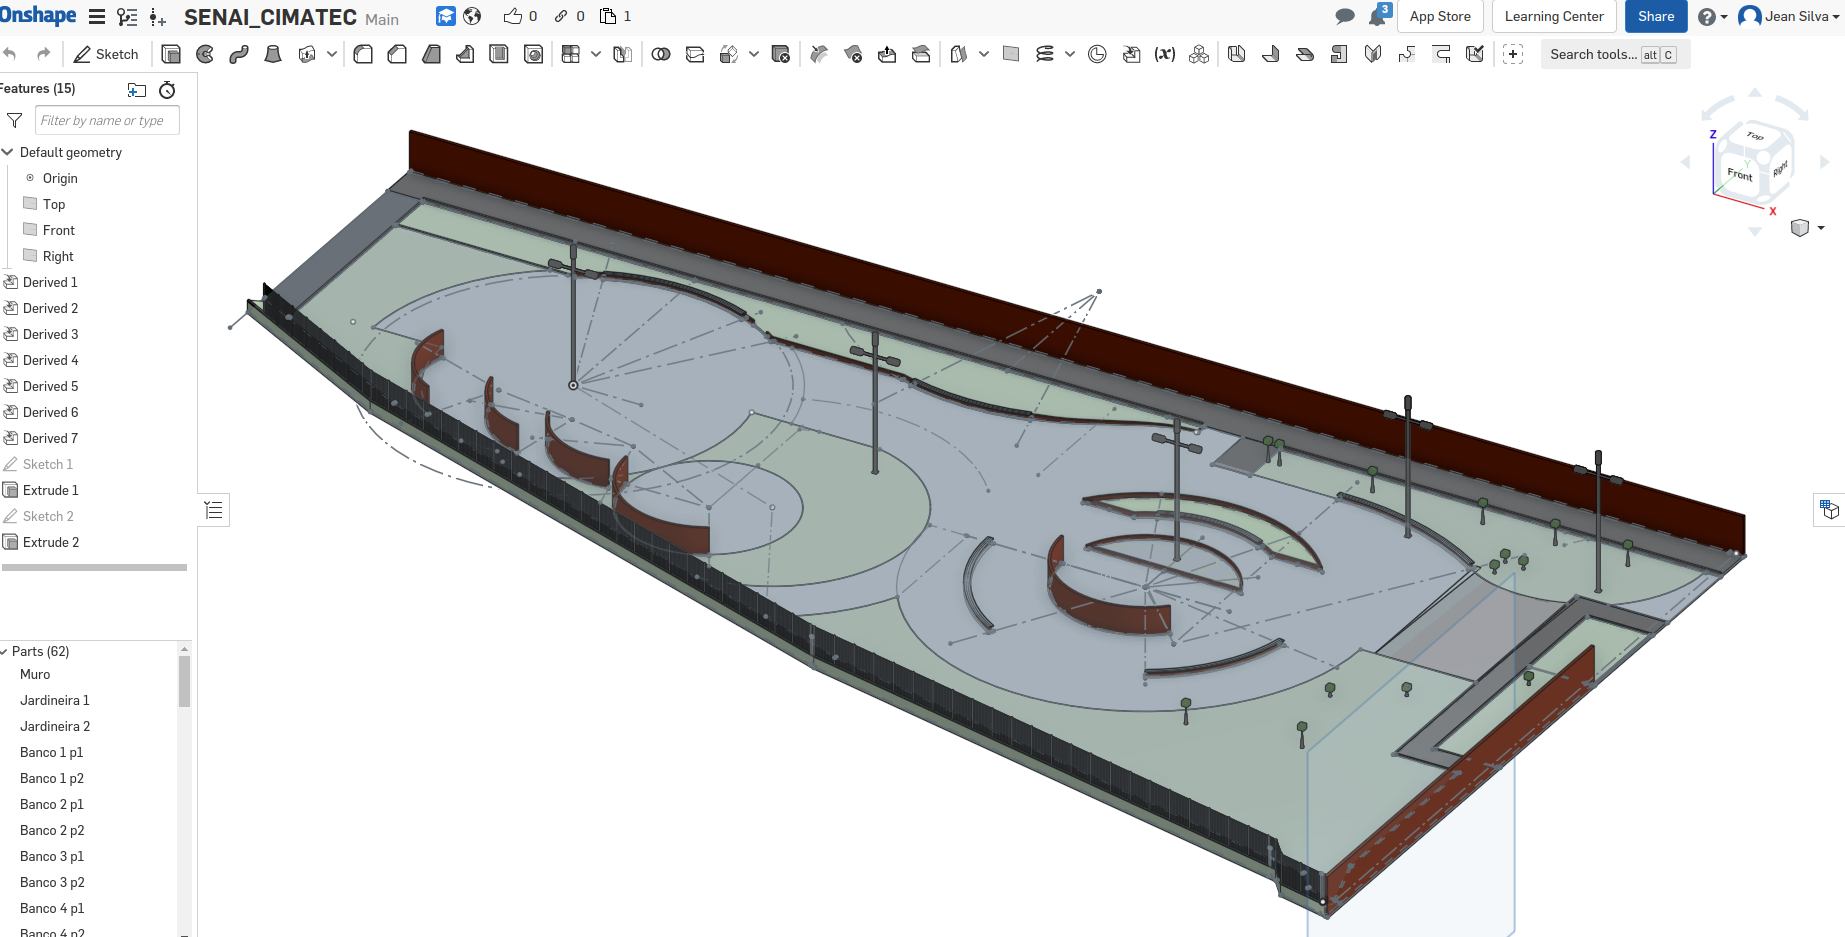
\includegraphics[width=1.0\textwidth]{./des1map}	
	\caption*{Fonte: Grupo de formação em Robótica e Sistemas Autônomos}		
	\label{img:des1map}									 
\end{figure}

\begin{figure} [H]												
    \centering
    \caption{Robô \textit{Clearpath Husky} simulado em ambiente \textit{Gazebo}.}										
	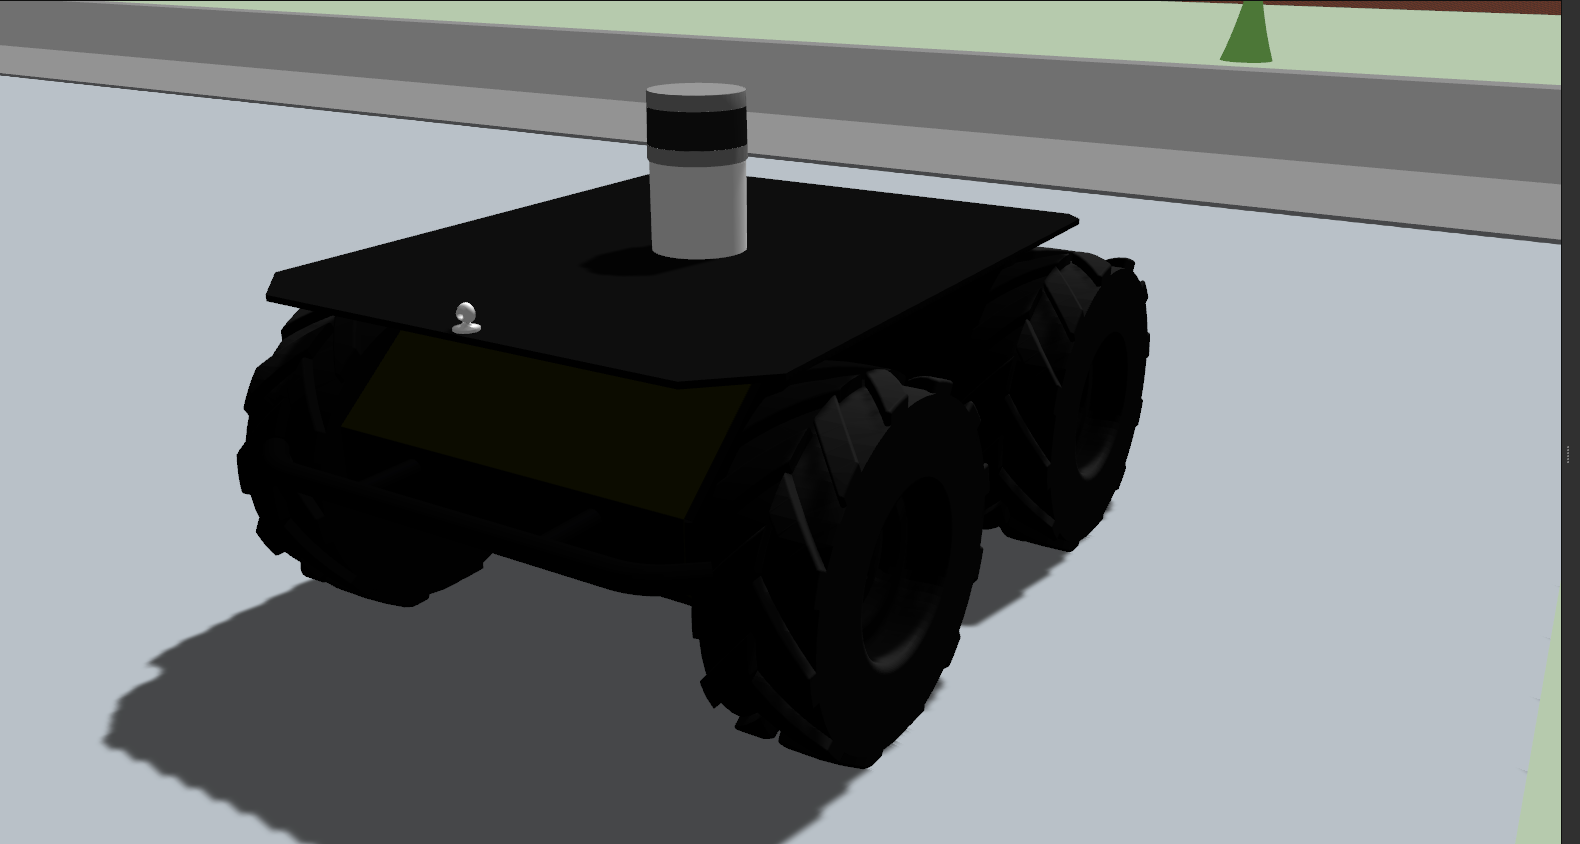
\includegraphics[width=1.0\textwidth]{./des1husky}	
	\caption*{Fonte: Grupo de formação em Robótica e Sistemas Autônomos}		
	\label{img:des1husky}									 
\end{figure}

\begin{figure} [H]												
    \centering
    \caption{Bola amarela no ambiente de trabalho simulado.}												
	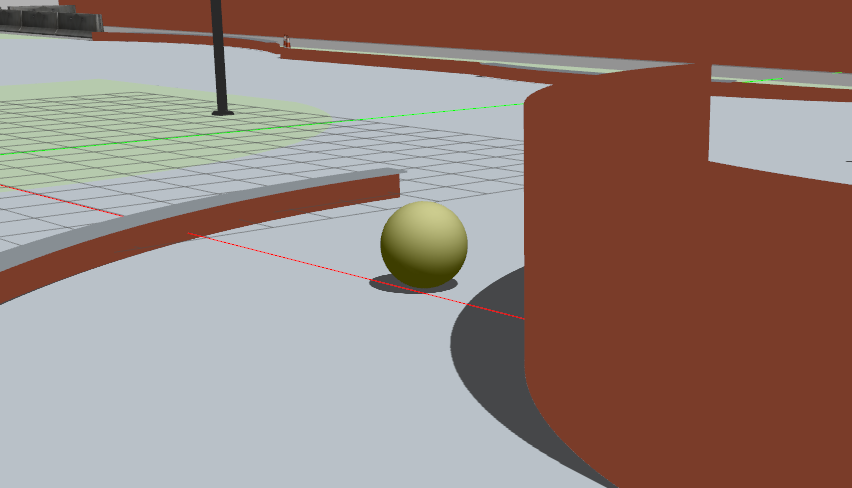
\includegraphics[width=1.0\textwidth]{./des1ball}	
	\caption*{Fonte: Grupo de formação em Robótica e Sistemas Autônomos}
	\label{img:des1ball}									 
\end{figure}
%----------------------------------------------------------

%--------- NEW SECTION ----------------------
\section{Desafio 2.0 - Entrega parcial: simulação do manipulador robótico RAJA}
\label{sec:des2}

Este desafio foi realizado em grupo de 4 pessoas e consistiu na simulação em \textit{Gazebo} de um manipulador robótico com 5 graus de liberdade de nome RAJA. Ele possui uma câmera \textit{RGB (Red, Green and Blue)} que tem finalidade em encontrar a posição de um botão de uma caixa no seu ambiente de trabalho. Esta posição é definida por um marcador fiducial \textit{ArUco (Augmented Reality by University of Cordoba)} que a caixa possui. Com a posição encontrada, o manipulador pressiona o botão com sua ferramenta. Todos os modelos simulados foram feitos no \textit{OnShape}. A Figura \ref{img:des2} representa o manipulador em seu ambiente de trabalho ao chegar até o botão. O Apêndice \ref{append:raja} representa o relatório deste desafio com suas especificações, arquitetura, desenvolvimento, metodologia e resultados.

\begin{figure} [H]												
    \centering
    \caption{Manipulador RAJA finalizando a missão.}	
	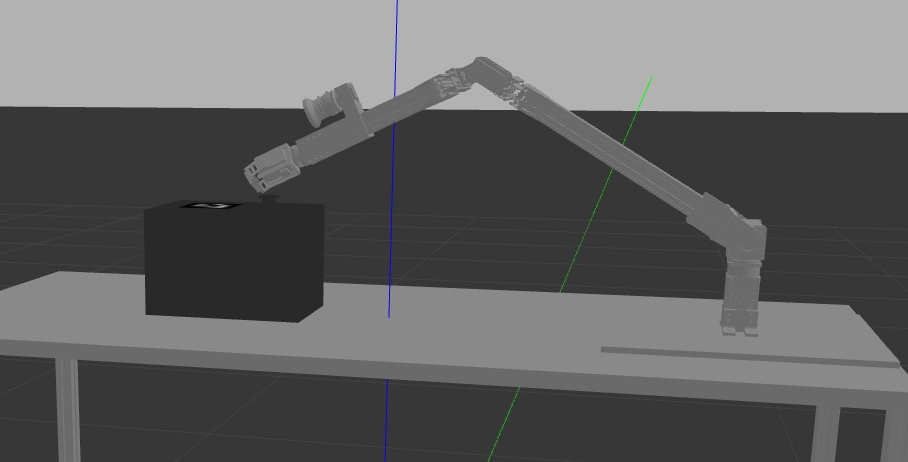
\includegraphics[width=1.0\textwidth]{./des2}	
	\caption*{Fonte: Grupo de formação em Robótica e Sistemas Autônomos}
	\label{img:des2}									 
\end{figure}

%--------- NEW SECTION ----------------------
\section{Desafio 2.2 - Entrega final do manipulador JeRoTIMON}
\label{sec:des22}

Este desafio realizado em um grupo de 6 pessoas, visou construir um modelo físico de um manipulador robótico baseado nos conceitos aplicados no desafio 2.0 (Subseção \ref{sec:des2}). Os objetivos continuaram os mesmos: obter a posição de um botão em uma caixa baseado em um marcador fiducial \textit{ArUco} utilizando uma câmera \textit{RGB} modelo \textit{Teledyne Genie Nano C2590} e pressioná-lo utilizando o manipulador robótico. A construção física do manipulador foi realizada com os materiais disponíveis no laboratório de Robótica e Sistemas Autônomos do SENAI CIMATEC. Sua base foi feita de madeira com suportes de aço, e os elos foram feitos com alumínio. Os motores são de marca ROBOTIS e modelos Dynamixel PLUS. A peça de suporte para a câmera foi feita a partir de impressão 3D com material ABS. A Figura \ref{img:des22} mostra o manipulador em seu ambiente de trabalho com a caixa objetivo. No Apêndice \ref{append:jerotimon} está disponível o relatório com maiores detalhes sobre o desenvolvimento, metodologia e resultados.

\begin{figure} [H]												
    \centering
    \caption{Manipulador JeRoTIMON no ambiente de trabalho e a caixa objetivo.}	
	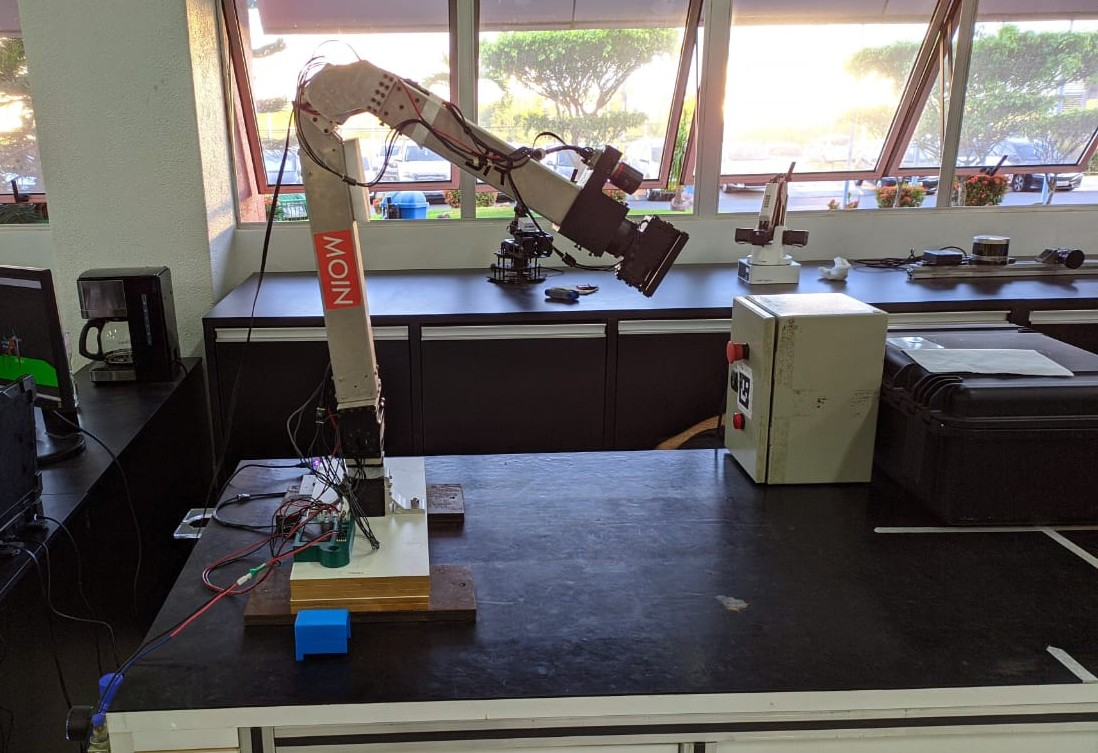
\includegraphics[width=1.0\textwidth]{./des22}	
	\caption*{Fonte: Grupo de formação em Robótica e Sistemas Autônomos}
	\label{img:des22}									 
\end{figure}


%--------- NEW SECTION ----------------------
\section{Desafio 2.5 - Análise estatística R\&R do robô Darwin-OP}
\label{sec:des25}

Este desafio foi realizado em um grupo de 4 pessoas, as mesmas do desafio \ref{sec:des2}. O objetivo deste trabalho era desenvolver um ambiente simulado em \textit{Gazebo}, e realizar ações autônomas de marcha liderada e corrida de revezamento com 4 robôs humanóides \textit{Darwin-OP} (Figura \ref{img:darwin}). Na marcha liderada, os 4 robôs devem andar em velocidade sincronizada durante 2 metros, como mostra a Figura \ref{img:marcha}. Na corrida de revezamento, cada robô está posicionado em uma parte específica da pista de corrida (Figura \ref{img:revezamento}), em que ele deve aguardar o robô anterior se aproximar, manter-se próximo em velocidade sincronizada por cerca de 5 segundos (representando a passagem de bastões) e depois seguir em maior velocidade para alcançar o robô à sua frente. A pista projetada pode ser visualizada na Figura \ref{img:pista}.

Este projeto teve um estudo estatístico que pode ser visto no Apêndice \ref{append:darwin}, e tem por objetivo analisar a medição dos dados utilizando o método de análise de variância.

\begin{figure} [H]												
    \centering
    \caption{\textit{Darwin-OP} em ambiente simulado.}	
	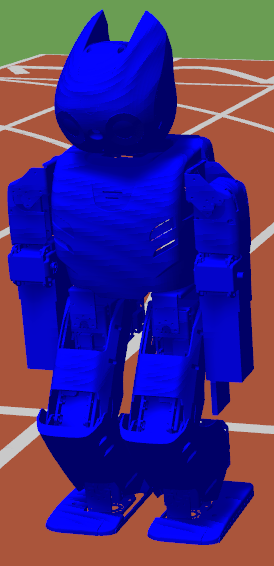
\includegraphics[width=0.6\textwidth]{./darwin-op}	
	\caption*{Fonte: Grupo de formação em Robótica e Sistemas Autônomos}
	\label{img:darwin}									 
\end{figure}

\begin{figure} [H]												
    \centering
    \caption{\textit{Darwin-OP} em posição de marcha liderada.}	
	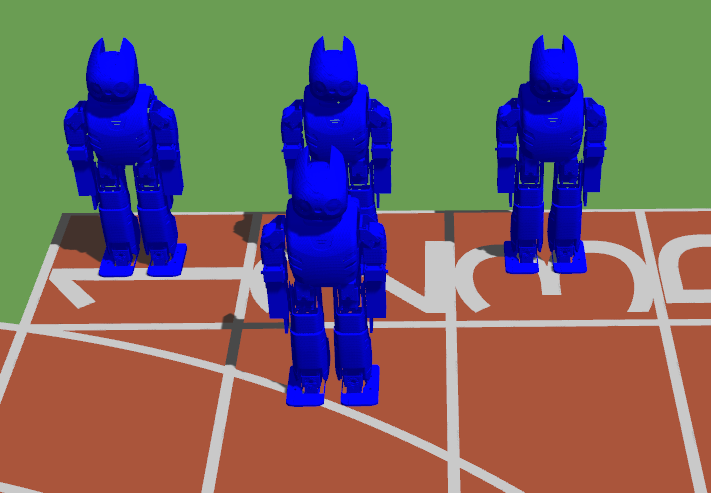
\includegraphics[width=1.0\textwidth]{./ordunmarcha}	
	\caption*{Fonte: Grupo de formação em Robótica e Sistemas Autônomos}
	\label{img:marcha}									 
\end{figure}

\begin{figure} [H]												
    \centering
    \caption{\textit{Darwin-OP} em posição de revezamento.}	
	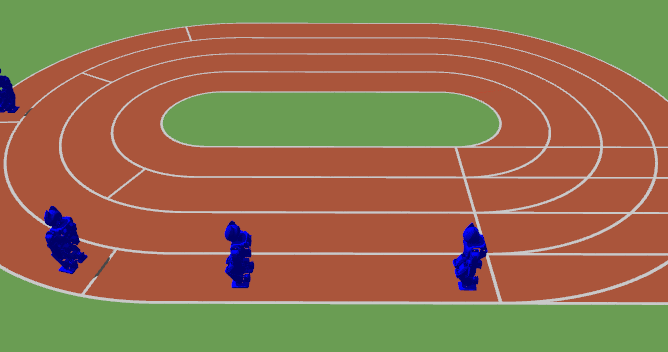
\includegraphics[width=1.0\textwidth]{./visao-darwin}	
	\caption*{Fonte: Grupo de formação em Robótica e Sistemas Autônomos}
	\label{img:revezamento}									 
\end{figure}

\begin{figure} [H]												
    \centering
    \caption{Pista e suas dimensões.}	
	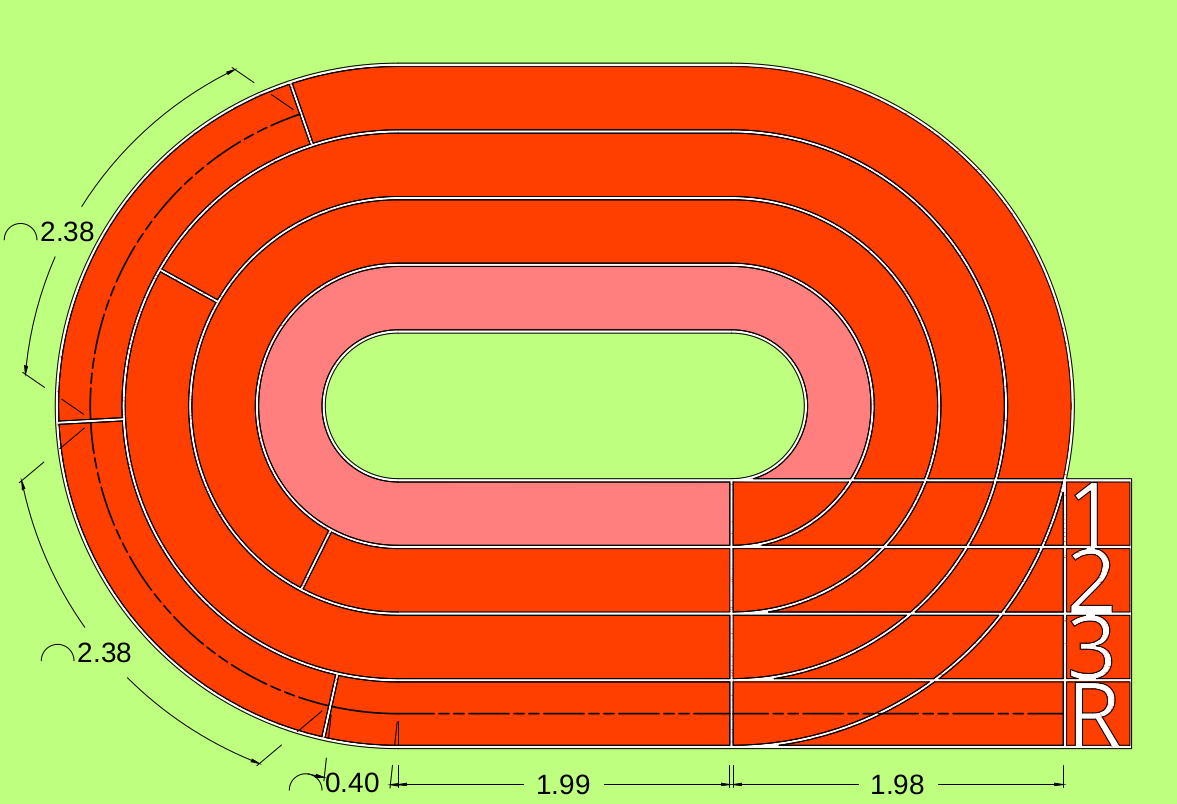
\includegraphics[width=1.0\textwidth]{./track}	
	\caption*{Fonte: Grupo de formação em Robótica e Sistemas Autônomos}
	\label{img:pista}									 
\end{figure}

%--------- NEW SECTION ----------------------
\section{Desafio 3.0 - Curupira}
\label{sec:des3}

Este desafio foi realizado por um grupo de 3 pessoas. O projeto Curupira representa a integração do \textit{UGV Clearpath Robotics Warthog} e o manipulador JeRoTIMON, visto na Subseção \ref{sec:des22}. Equipado com sensores para as funcionalidades de percepção de localização, como câmera \textit{RGB}, \textit{LIDAR (Light Detection and Ranging)} e \textit{GPS (Global Positioning System)}, o objetivo é dar autonomia ao sistema para que ele consiga identificar uma ``bomba'' (Figura \ref{img:bomba}) presente em um lugar aleatório da área externa ao CIMATEC 4 (visto na Figura \ref{img:des1mapreal} na Subseção \ref{sec:des1}). A posição do objetivo é adquirida pela câmera, e o objetivo é considerado completo quando o manipulador tocar nos fios da ``bomba''.

Este projeto foi dividido em duas partes: simulada em ambiente \textit{Gazebo}; e a construção real da integração, visto na Figura \ref{img:curupira}. O desenvolvimento, metodologia e resultados podem ser vistos no Apêndice \ref{append:curupira}.

\begin{figure} [H]												
    \centering
    \caption{``Bomba'' identificada pela rede neural no ambiente de trabalho.}	
	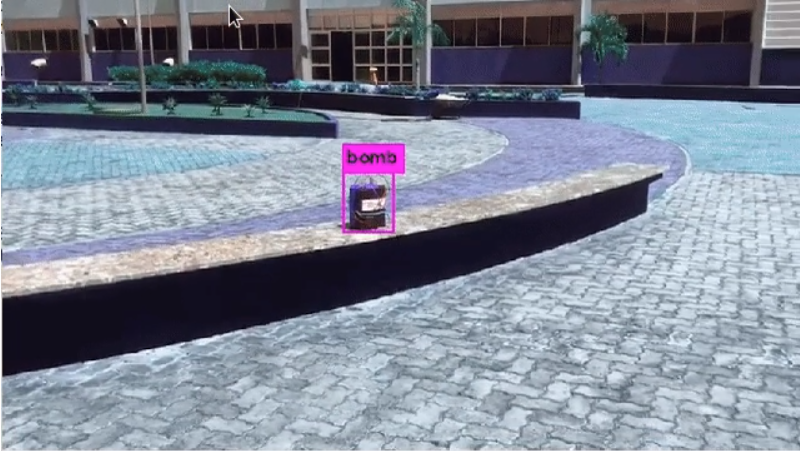
\includegraphics[width=0.8\textwidth]{./int-detection2}	
	\caption*{Fonte: Grupo de formação em Robótica e Sistemas Autônomos}
	\label{img:bomba}									 
\end{figure}

\begin{figure} [H]												
    \centering
    \caption{Integração física.}	
	\includegraphics[width=0.55\textwidth]{./modularidade}	
	\caption*{Fonte: Grupo de formação em Robótica e Sistemas Autônomos}
	\label{img:curupira}									 
\end{figure}

%--------- NEW SECTION ----------------------
\section{Estudo estatístico de \textit{DOE (Design of Experiments)}}
\label{sec:doe}

Este desafio foi realizado em um grupo de 4 pessoas, as mesmas do desafio \ref{sec:des2}. O objetivo deste experimento foi aplicar os conceitos de estatística aprendidos durante a especialização. Foi utilizado um modelo de helicóptero de papel em um experimento de medição do seu tempo de queda. Durante o processo de medição, foram adicionados adesivos e clipes ao helicóptero, modificando seu tempo de queda. Os conceitos de \textit{DOE} foram aplicados para identificar quais os fatores mais influenciam a variável controlada: tempo de vôo. Esta análise foi feita utilizando o \textit{software} estatístico \textit{R Studio} para tratamento dos dados e visualização final. Os resultados e interpretações estão no Apêndice \ref{append:doe}.
    \chapter{Metodologia}
\label{chap:mat}

Um dos pontos característico do programa de Formação em Robótica é a sua metodologia, onde buscará a aprendizagem ativa do estudante, com a construção dos seus conhecimentos, complementando as aulas expositivas com atividades e dinâmicas de grupo, elaboração e apresentação de trabalhos e pesquisas, emprego de meios audiovisuais, estudos individualizados, pesquisa de artigos técnicos e científicos, entre outros condicionantes ao programa.
A metodologia em si é um caminho para o sucesso na formação dos estudantes, pois esta convergência baseia-se em 5 pontos principais:

\begin{enumerate}
    \item \textbf{Criatividade:} espaço que estimula a criatividade, possibilitando interação e acesso à diferentes tecnologias.
    \item \textbf{Engajamento:} atividades práticas de aprendizado aumentam os níveis de concentração
    \item \textbf{Programação:} a inteligência artificial se torna cada vez mais presente nas escolas e escritórios
    \item \textbf{Trabalho em equipe:} robótica incorpora uma gama de habilidades e promove um ambiente de aprendizagem para pessoas com diferentes talentos
    \item \textbf{Diversão:} aprender sobre robótica deve ser divertido, e a medida que os estudantes continuem melhorando sua interação com eles, isso aumenta mais ainda o nível de diversão
\end{enumerate}


Basicamente o caminho para o sucesso compreende em 4 fases distintas, demonstradas na Figura \ref{fig:metodologia}:

\textbf{Assimilação:} desenvolver habilidades de codificação e lógica;

\textbf{Simulação:} testar as missões de um robô de forma eficiente;

\textbf{Integração:} garantir informações sobre o ambiente e o robô;

\textbf{Criação:} elaborar um projeto aplicado a tecnologia.

As três primeiras fases são compreendidas em 6 meses, ficando a fase Criação com 6 meses para finalizar o programa.
Entre cada fase, desafios são lançados para que o estudante obtenha maior sucesso na assimilação dos conceitos ministrados, para a última fase um projeto final é lançado para que o estudante possa realizar a demonstração de seu sistema para os avaliadores.
Bom salientar que durante as fases, temas serão tratados e discutidos de forma expositiva e prática.


\begin{figure}[H]
    \caption{Metodologia do Programa de Formação em Robótica e Sistemas Autônomos}
    \centering
    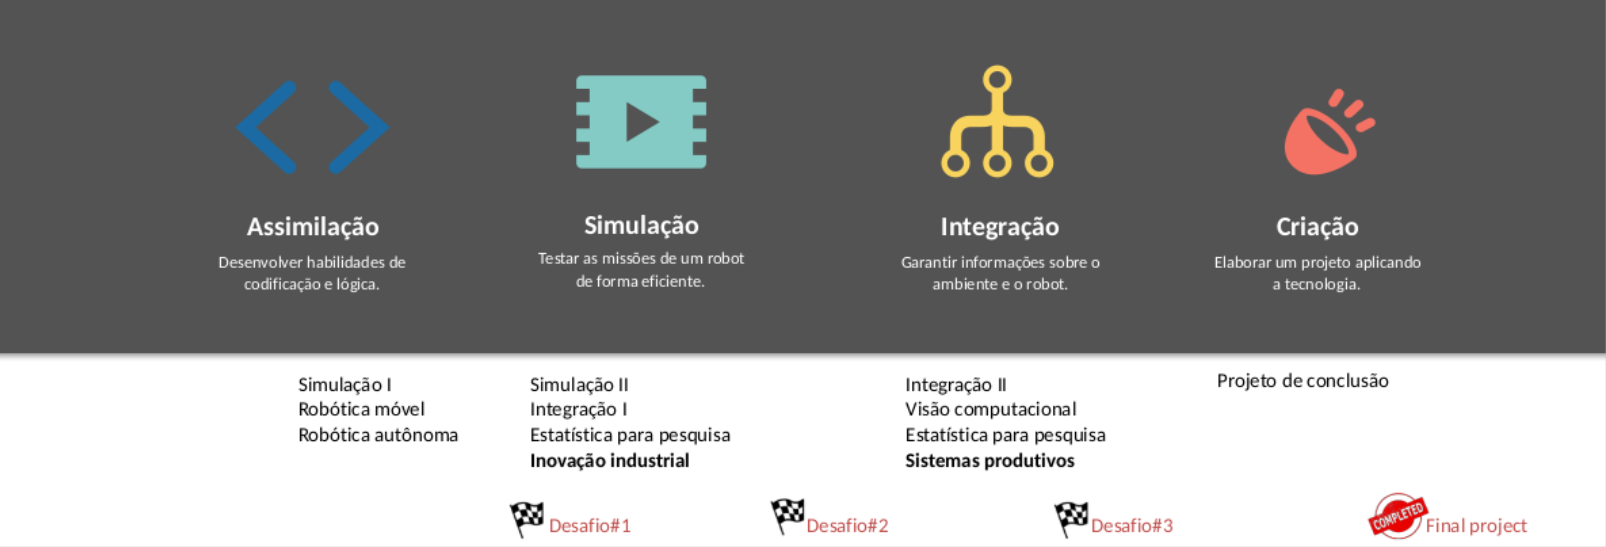
\includegraphics[width= \textwidth]{Figures/metodologia.png}
    \caption*{Fonte: Programa de Formação em Robótica e Sistemas Autônomos}
    \label{fig:metodologia}
\end{figure}

Com uma abordagem inovadora, o programa tenta realçar a busca por um aprendizado mais real e excitante para isso o conceito de professor facilitador que estimule a experiência nas várias tecnologias se faz necessário. Isso promoverá vários feedbacks mais intensos aos estudantes. Em resumo o professor será o facilitador de uma experiência de aprendizado, criando recursos e experiência para a formação do aprendiz.
    \chapter{Resultados}
\label{chap:result}
Neste capítulo são expostos os resultados provenientes dos artigos desenvolvidos baseados nos desafios e entregas que foram expostos nos eventos SAPCT (Seminário de Avaliação de Pesquisa Científica e Tecnologia) e SIINTEC (Simpósio Internacional de Inovação e Tecnologia) de 2020.

%--------- NEW SECTION ----------------------
\section{Resultado do Artigo RAJA: MANIPULADOR ROBÓTICO DE 5 DOF COM DETECÇÃO VISUAL INTEGRADA}
\label{sec:sapct}
Para o V SAPCT e IV ICPAD (Integração e Capacitação em Processamento de Alto Desempenho), o artigo baseado no projeto do manipulador robótico RAJA, visto no Apêndice \ref{append:rajamanip}, foi enviado e aceito pelo evento. Este projeto recebeu o prêmio de melhor trabalho na categoria PD\&I (Pesquisa, Desenvolvimento e Inovação), e o certificado pode ser visto no Apêndice \ref{append:sapct}.

\section{Resultado do Artigo PERSPECTIVES ON AUTONOMOUS UNMANNED GROUND VEHICLES: A SURVEY}
\label{sec:siintec}

Este resultado foi baseado no projeto conceitual de dois UGVs. Os veículos possuem dois portes: o de porte médio, de nome Capivara;  e outro de porte pequeno, de nome Mocó - ambos homenageando a fauna brasileira. Ambos possuem a finalidade de aspersão de ambientes, tendo em visto o contexto da pandemia causada pelo Coronavírus. O Seminário foi apresentado no evento SIINTEC 2020. Seu artigo pode ser visto no Apêndice  \ref{append:artsiintec} e a certificação gerada pode ser visualizada no Apêndice \ref{append:siintec}. 








    \chapter{Conclusão}
\label{chap:conc}

O programa de formação Novos Talentos 2020 em Robótica e Sistemas Autônomos possibilitou a aprendizagem de habilidades e competências requeridas para trabalhar em projetos de robótica. Isso foi possível graças à metodologia empregada, que foca em fazer com que o bolsista aprenda os conhecimentos necessários por atividades práticas de maneira contínua e gradual. A metodologia trabalhada durante o programa contribuiu para uma maneira flúida de assimilamento de informações e os resultados apresentados no documento confirmam sua eficácia. A presença imediata de vários orientadores especialistas também é responsável por grande parte dos resultados obtidos durante a formação. Esta abordagem necessita de estímulos, correções e avaliações constantes; características presentes durante todo o processo.

Além dos conteúdos técnicos passados, houveram também ensinamentos sobre competências esperadas de um pesquisador trabalhando em projetos, como liderança, planejamento, trabalho em equipe, criatividade e gerenciamento. Os desafios e trabalhos desenvolvidos durante a formação contribuíram para a publicação de artigos e a participação de seminários, resultados fundamentais para a formação de um pesquisador, tornando o processo de formação extremamente gratificante e motivador.
    % include more chapters ...
%
% ----------------------------------------------------------------------------
% Include thesis appendices
    \begin{thesisappendices}
        % % Thesis Appendix -------------------------------------------------------

\chapter{Diagramas mecânicos}
\label{Append:diagmec}



        % % Thesis Appendix -------------------------------------------------------

\chapter{Diagramas eletro-eletrônicos}
\label{Append:diagele}


        % % Thesis Appendix -------------------------------------------------------

\chapter{Logbook}
\label{Append:log}




        \chapter{MANIPULADOR ROBÓTICO RAJA}
        \label{append:raja}
        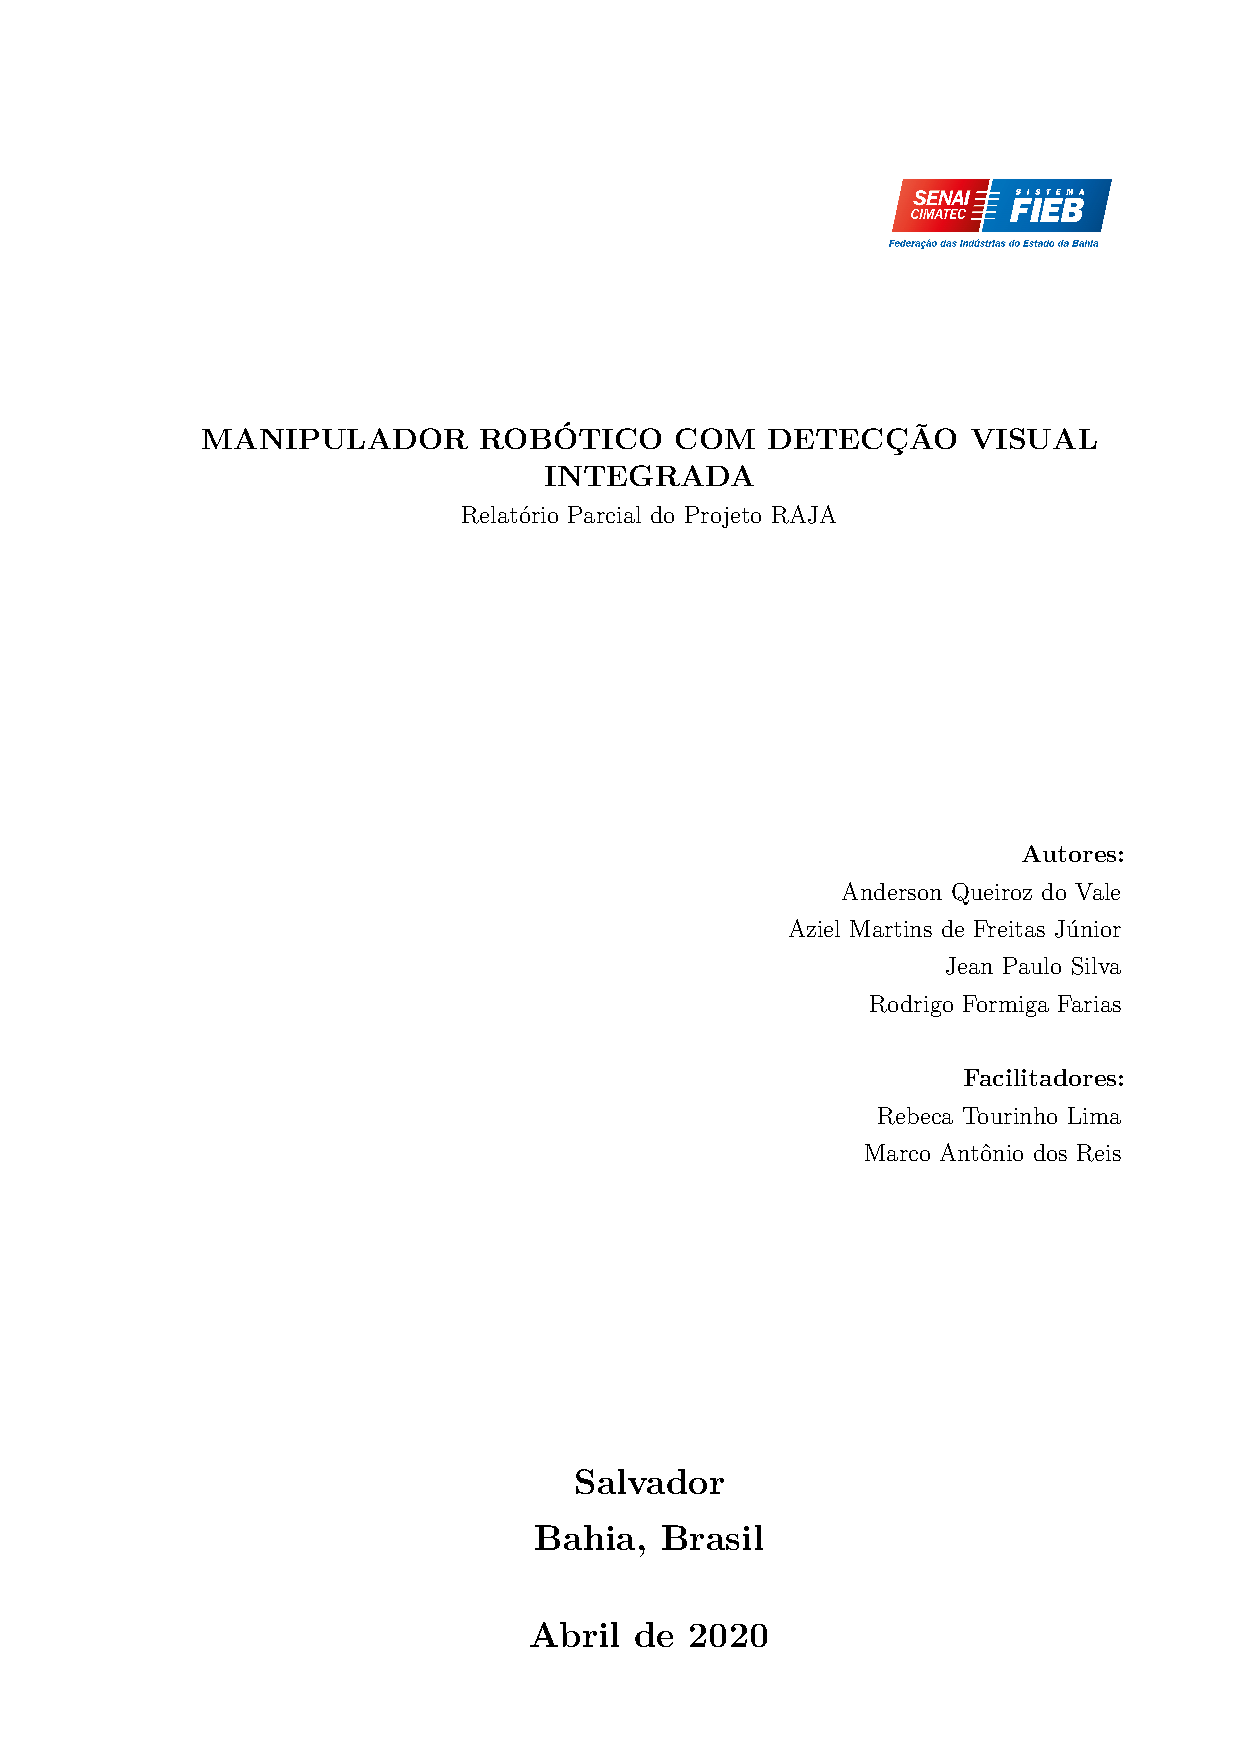
\includepdf[pages={1-66}, pagecommand={}]{Appendices/desafio2.pdf}

        \chapter{MANIPULADOR ROBÓTICO JEROTIMON}
        \label{append:jerotimon}
        \includepdf[pages={1-134}, pagecommand={}]{Appendices/desafio22.pdf}

        \chapter{Avaliação de medição para o desafio 2.5}
        \label{append:darwin}
        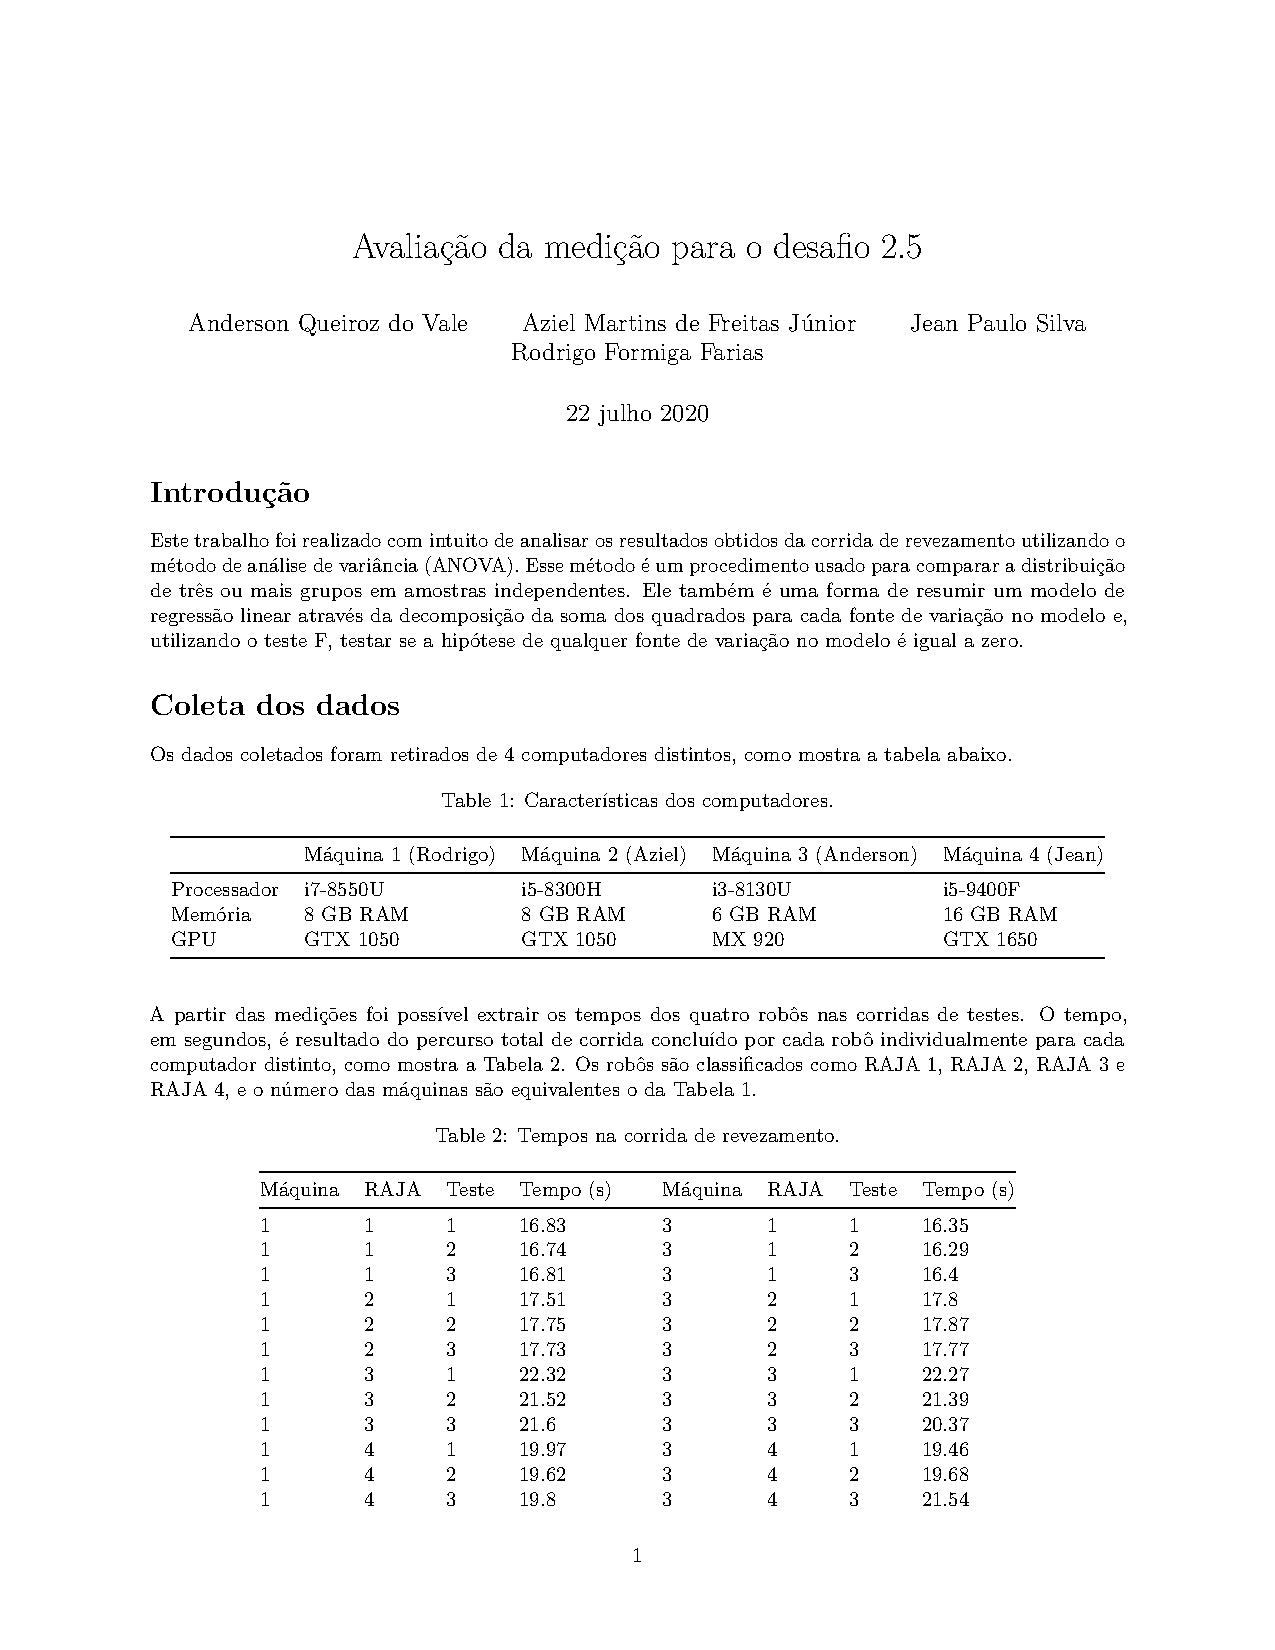
\includepdf[pages={1-5}, pagecommand={}]{Appendices/rajastats.pdf}

        \chapter{SISTEMA PARA IDENTIFICAÇÃO E MANIPULAÇÃO DE OBJETOS EM AMBIENTES EXTERNOS UTILIZANDO PLATAFORMA MÓVEL}
        \label{append:curupira}
        \includepdf[pages={1-115}, pagecommand={}]{Appendices/desafio3.pdf}

        \chapter{Estudo estatístico - Análise de Regressão}
        \label{append:doe}
        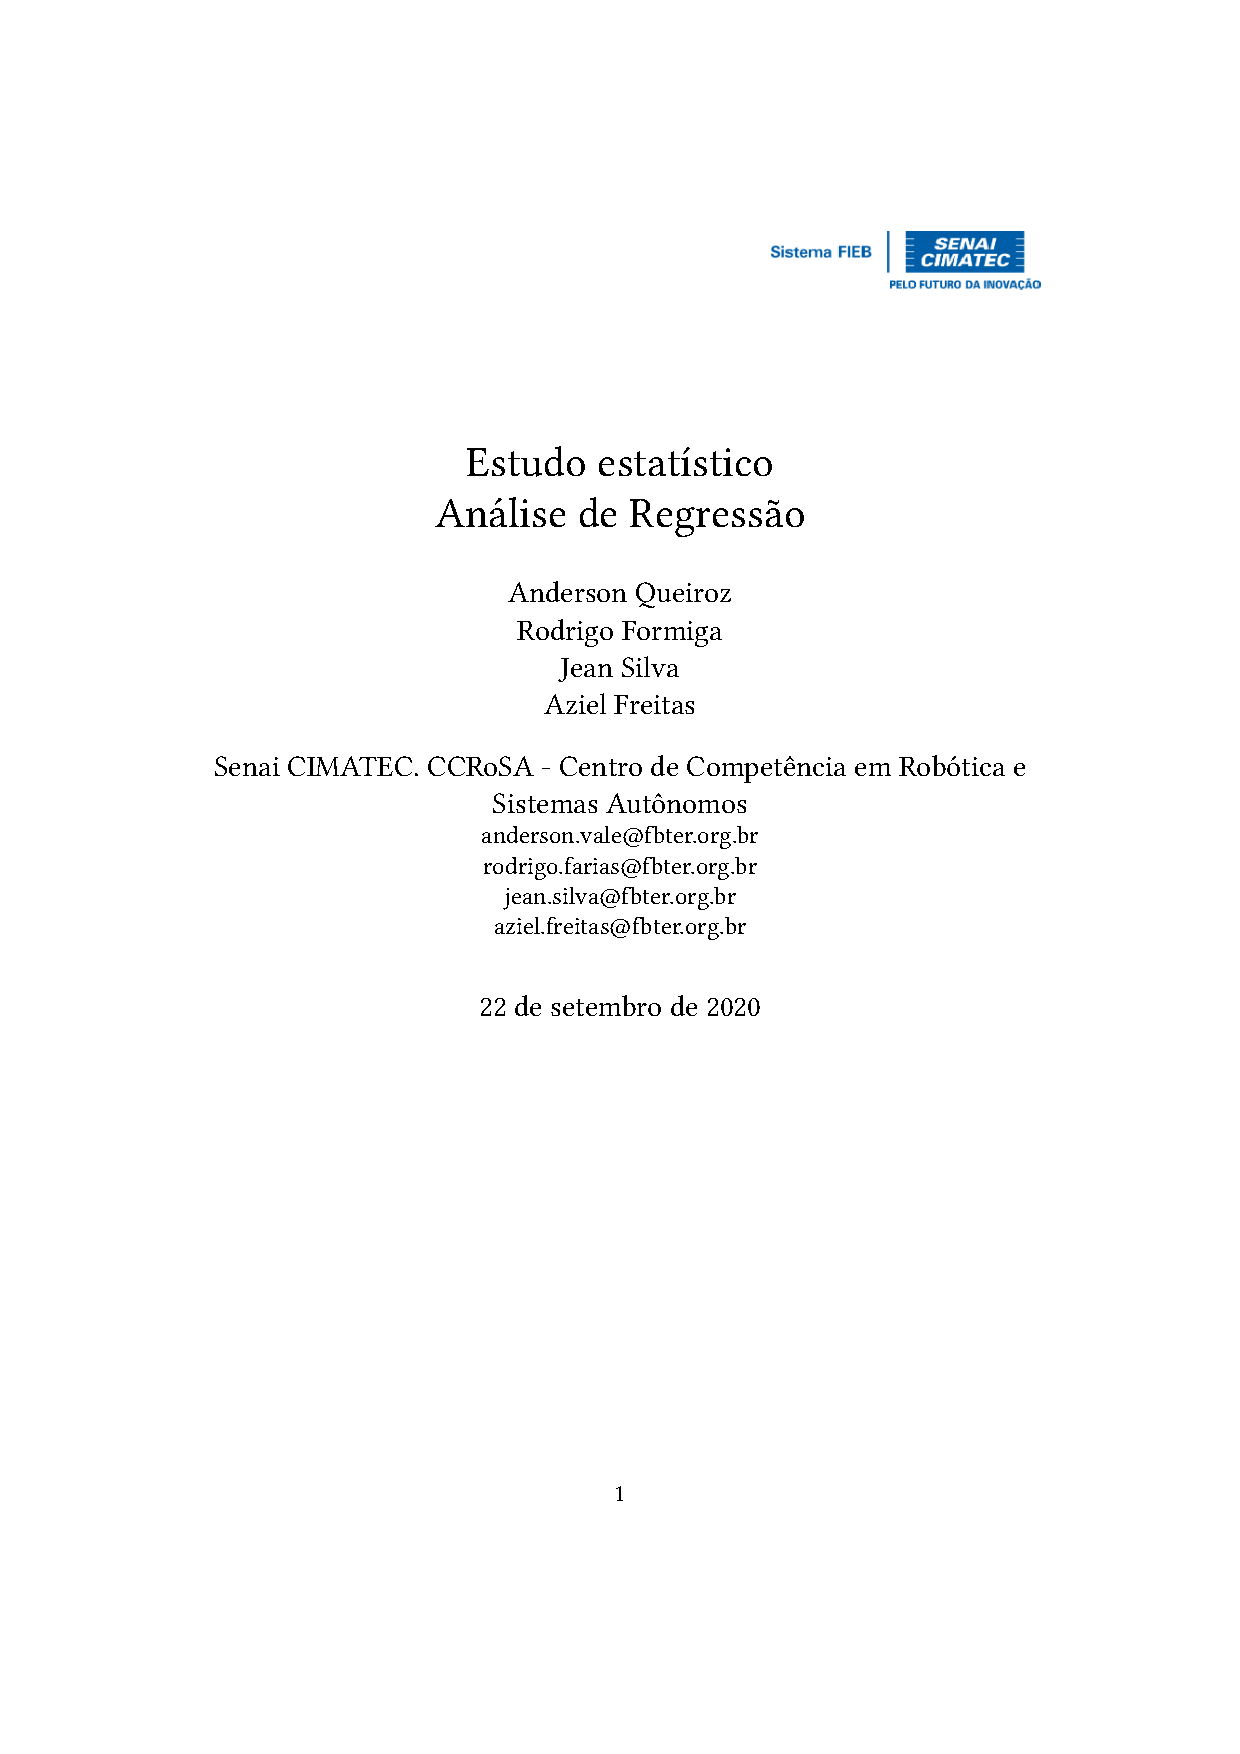
\includepdf[pages={1-19}, pagecommand={}]{Appendices/doe.pdf}

        \chapter{RAJA: MANIPULADOR ROBÓTICO DE 5 DOF COM DETEÇÃO VISUAL INTEGRADA}
        \label{append:rajamanip}
        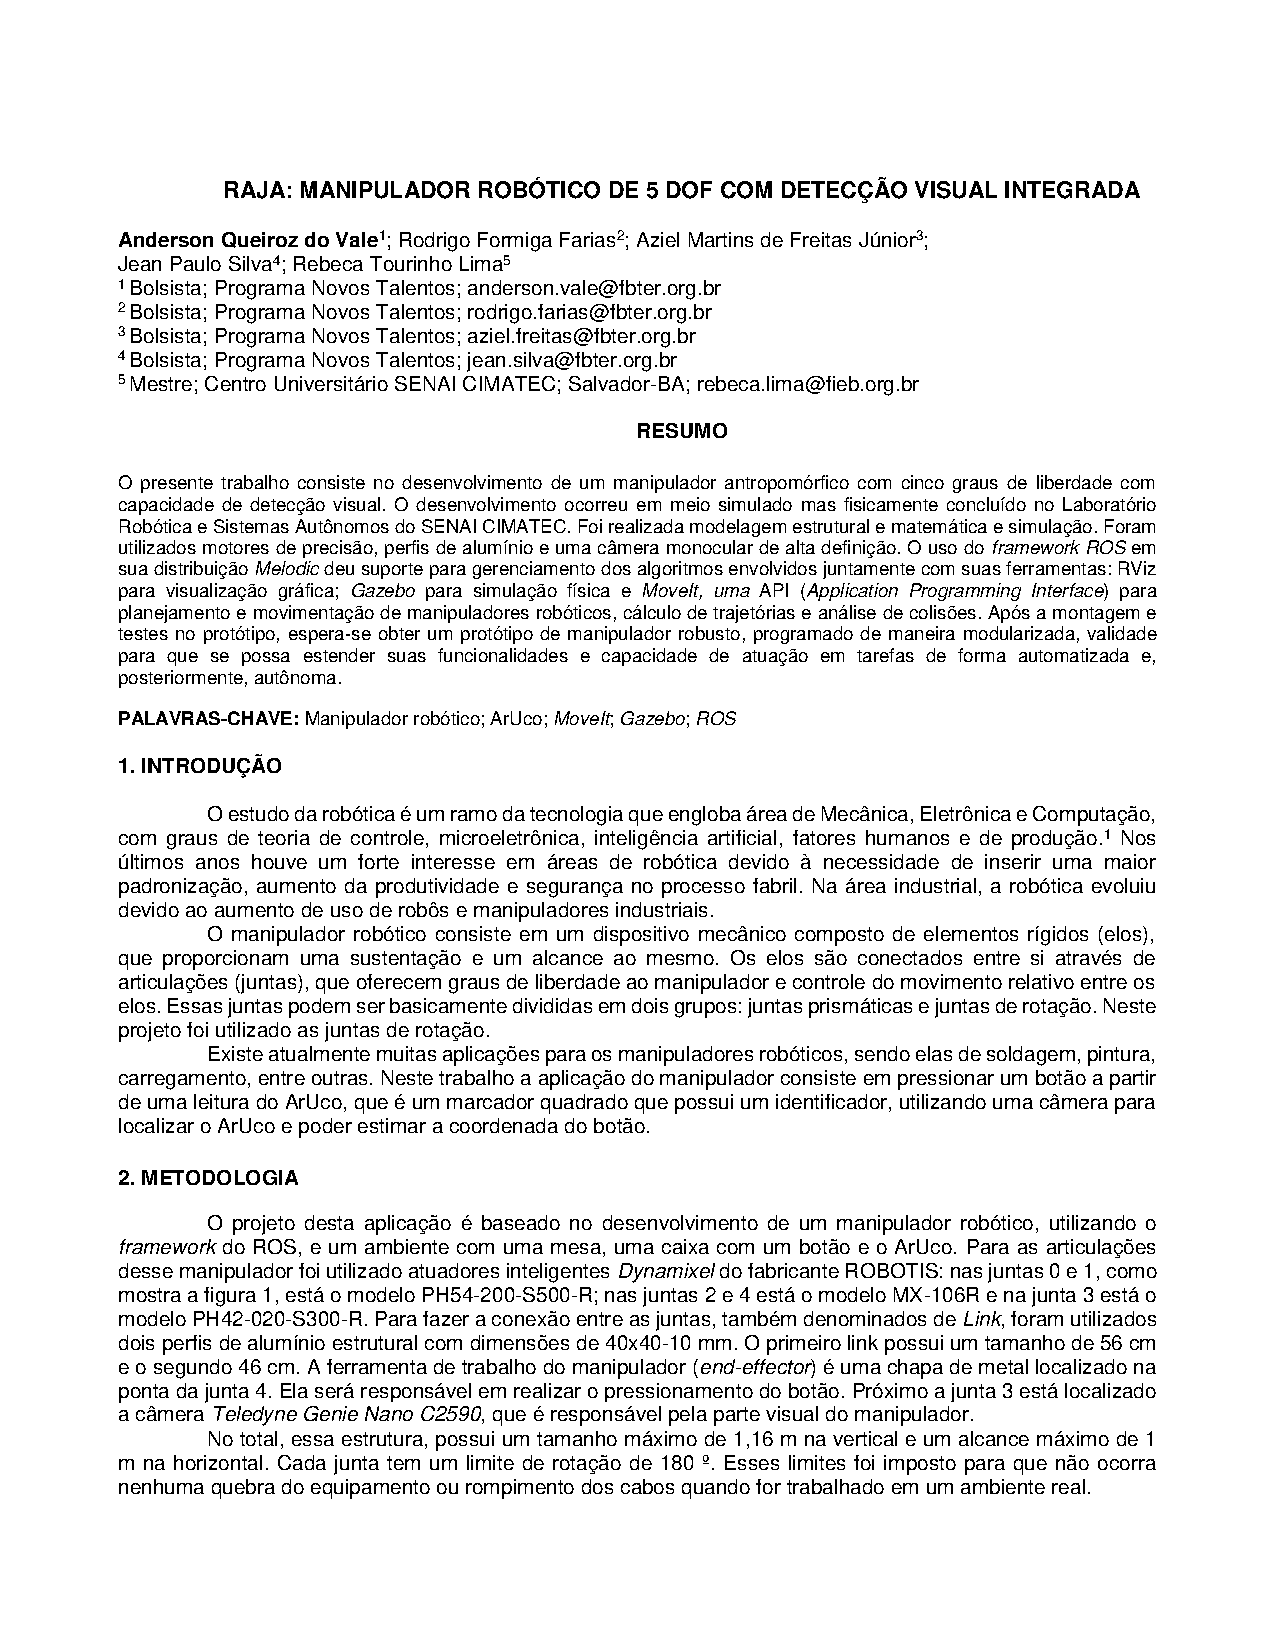
\includepdf[pages={1-3}, pagecommand={}]{Appendices/rajamanip.pdf}

        \chapter{Certificado de participação no V SAPCT}
        \label{append:sapct}
        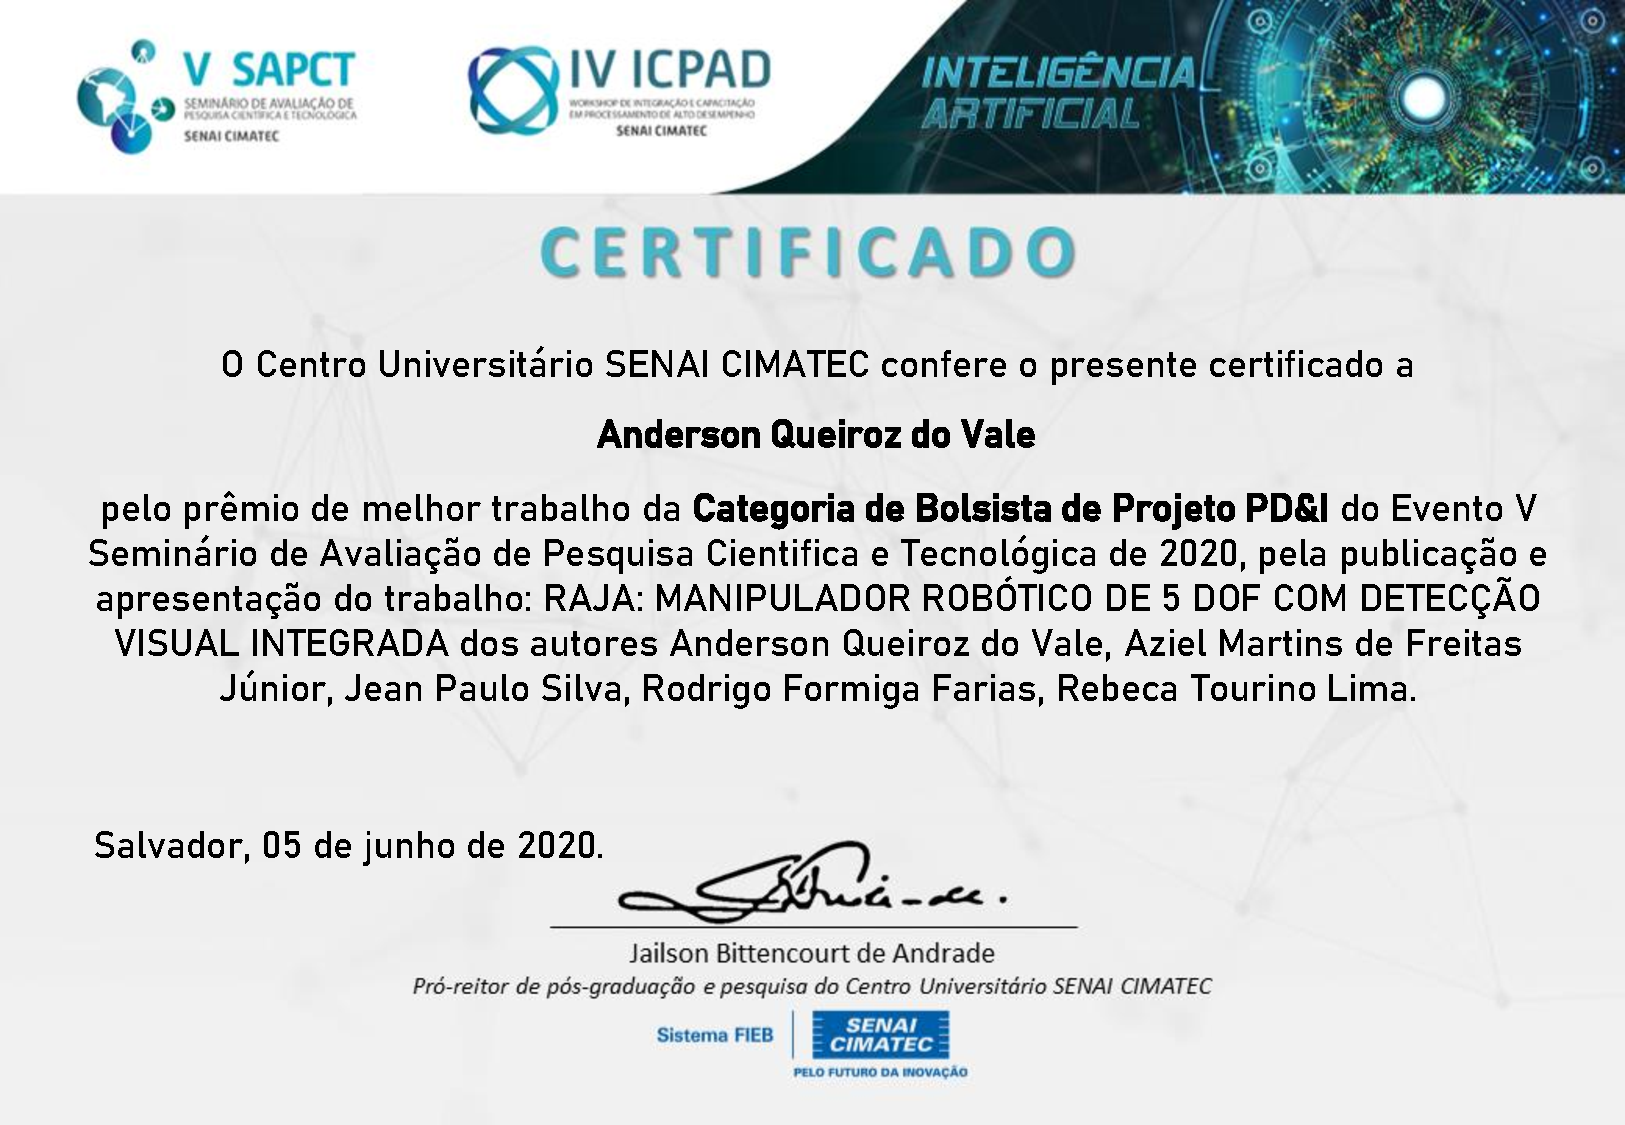
\includepdf[pages={1-1}, pagecommand={}]{Appendices/sapct.pdf}

        \chapter{PERSPECTIVES ON AUTONOMOUS UNMANNED GROUND VEHICLES: A SURVEY}
        \label{append:artsiintec}
        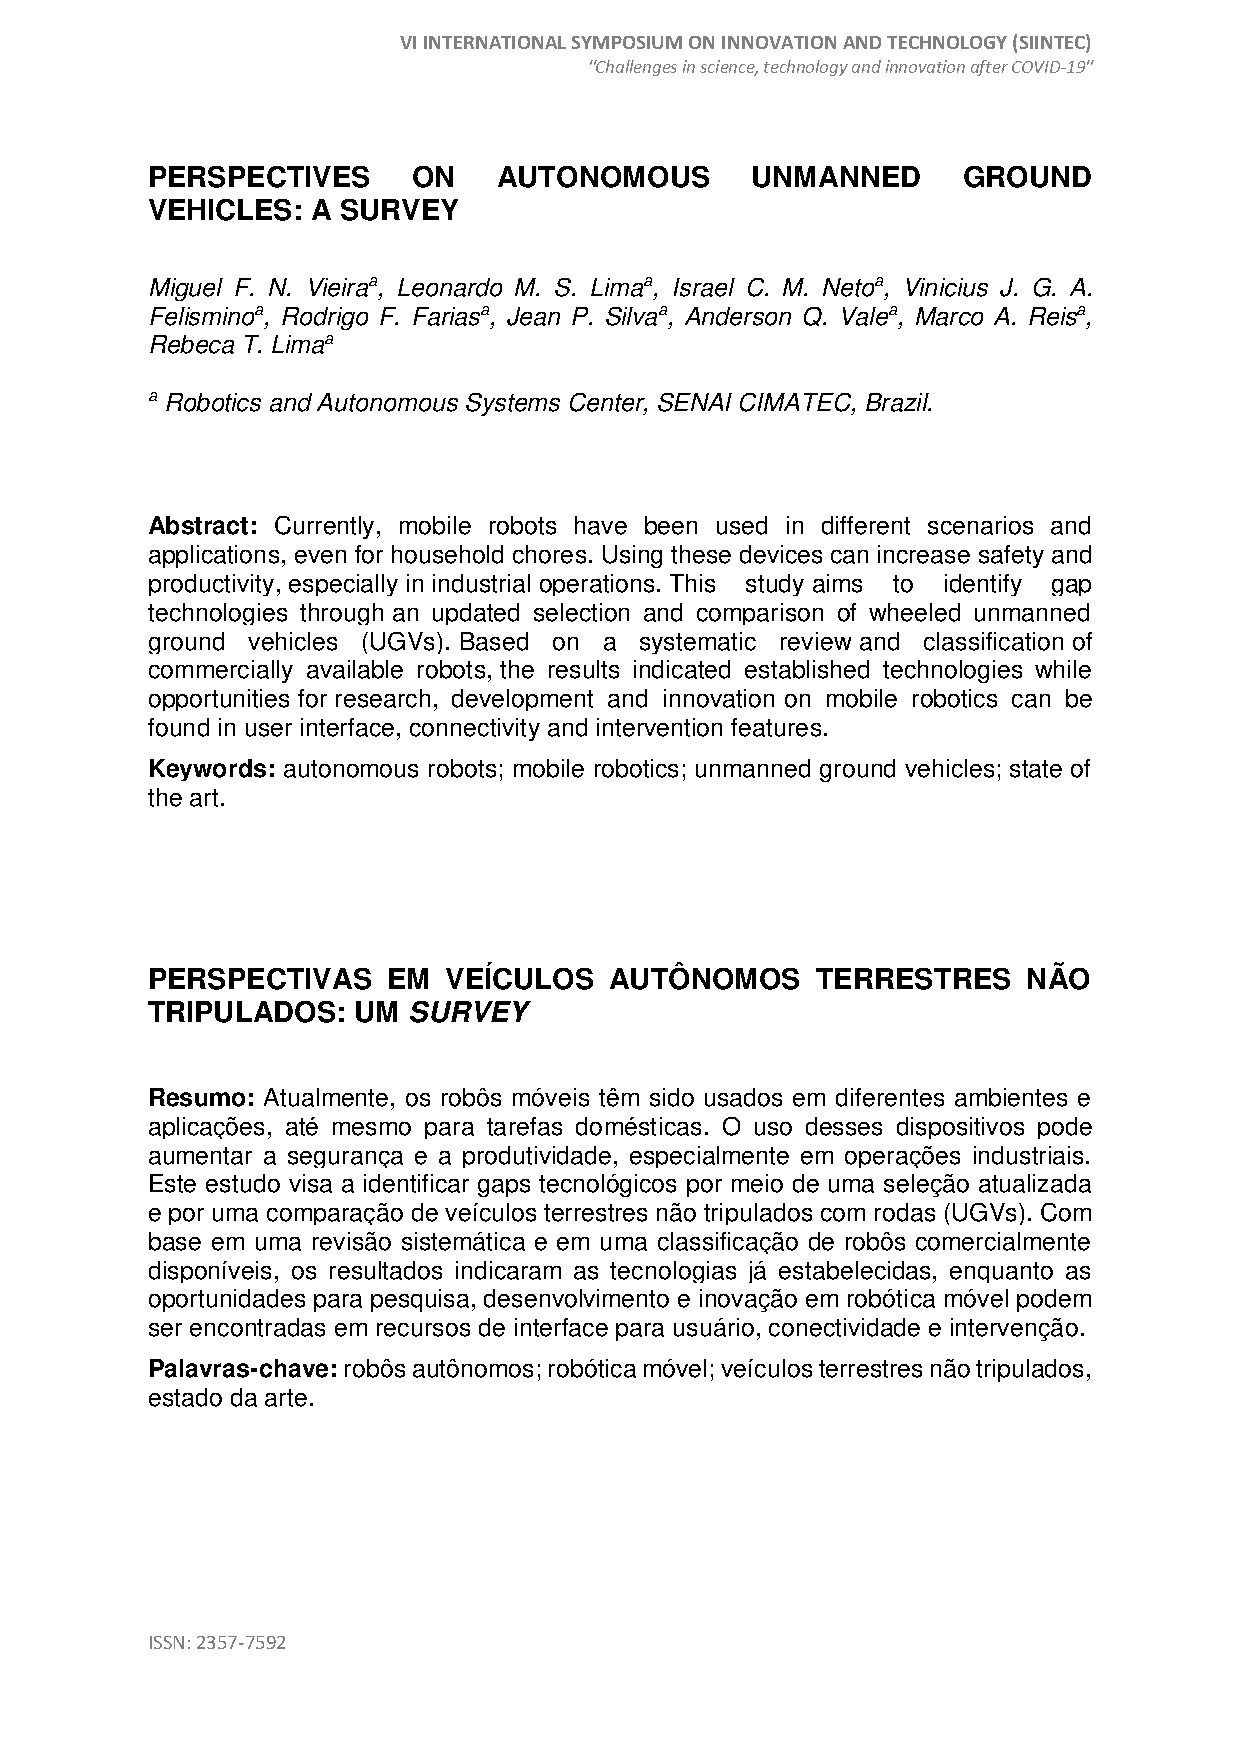
\includepdf[pages={1-8}, pagecommand={}]{Appendices/artsiintec.pdf}

        \chapter{Certificado de participação no VI SIINTEC}
        \label{append:siintec}
        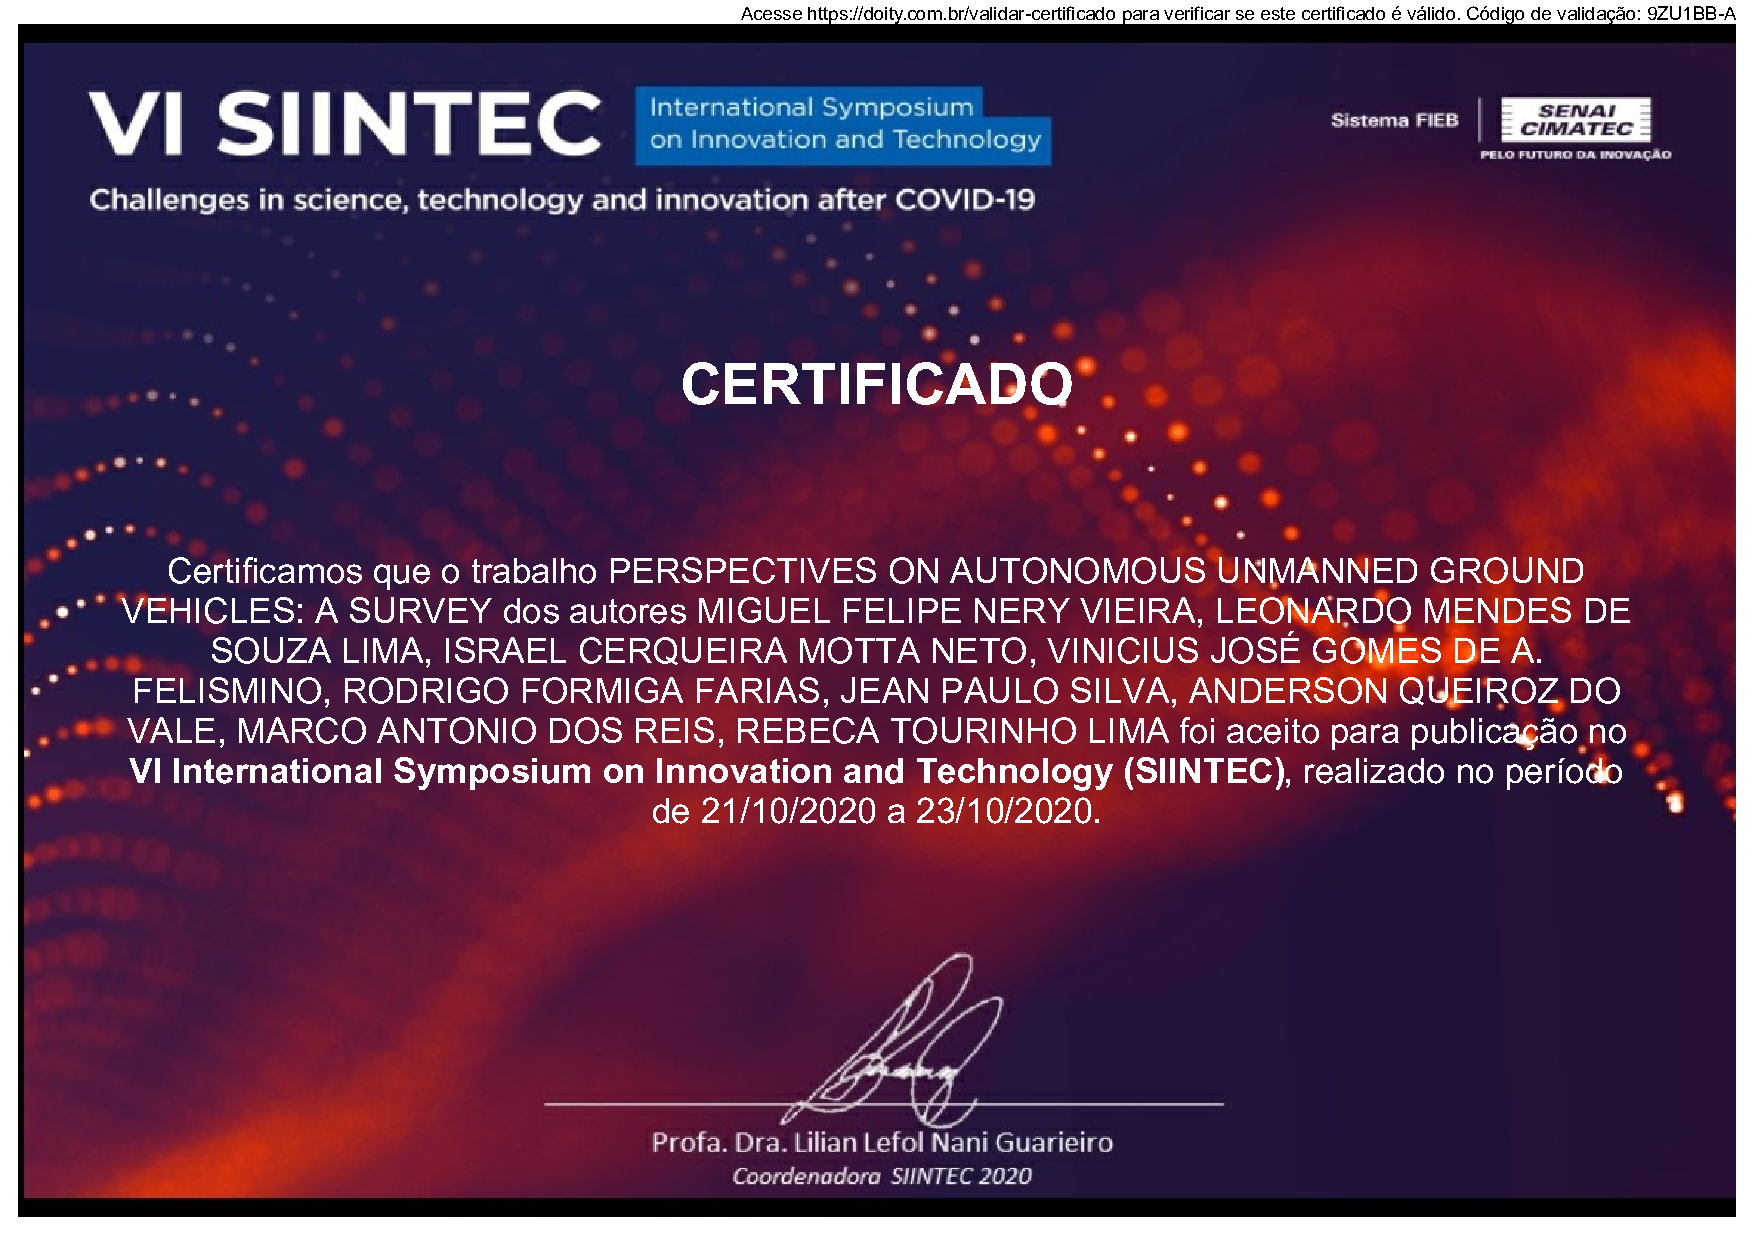
\includepdf[pages={1-1}, pagecommand={}]{Appendices/siintec.pdf}


    \end{thesisappendices}
%
% ----------------------------------------------------------------------------
% Configurar as referencias bibliograficas
	% \renewcommand\bibname{Referências}
    % \addcontentsline{toc}{chapter}{Referências}
    % \bibliography{References/referencias}
%
% ----------------------------------------------------------------------------
% Finishing him
    \include{Others/ultimafolha}
\end{document}
%
% -------------------------------------------------------------------------------
% Aqui termina a formatação para o documento.
% In God We Trust. All Other Bring Data. 
%
% -------------------------------------------------------------------------------